\documentclass[nobib]{tufte-handout}

%\\geometry{showframe}% for debugging purposes -- displays the margins

\newcommand{\bra}[1]{\left(#1\right)}
\usepackage{amssymb}
\usepackage{hyperref}
\usepackage[activate={true,nocompatibility},final,tracking=true,kerning=true,spacing=true,factor=1100,stretch=10,shrink=10]{microtype}
\usepackage{color}
\usepackage{steinmetz}
% Fixes captions and images being cut off
\usepackage{marginfix}
\usepackage{array}
\usepackage{tikz}
\usepackage{amsmath,amsthm}
\usetikzlibrary{shapes}
\usetikzlibrary{positioning}
\usepackage{listings}
\usepackage{caption}
\usepackage[americancurrents, americanvoltages, americanresistors, americaninductors]{circuitikz}
\DeclareCaptionFont{white}{\color{white}}
\DeclareCaptionFormat{listing}{\colorbox{gray}{\parbox{\textwidth}{#1#2#3}}}
\captionsetup[lstlisting]{format=listing,labelfont=white,textfont=white}

% Set up the images/graphics package
\usepackage{graphicx}
\setkeys{Gin}{width=\linewidth,totalheight=\textheight,keepaspectratio}
\graphicspath{{.}}

\title{ECE 20002: Electrical Engineering Fundamentals II}
\author[Zeke Ulrich]{Zeke Ulrich}
\date{\today}  % if the \date{} command is left out, the current date will be used

% The following package makes prettier tables.  We're all about the bling!
\usepackage{booktabs}

% The units package provides nice, non-stacked fractions and better spacing
% for units.
\usepackage{units}

% The fancyvrb package lets us customize the formatting of verbatim
% environments.  We use a slightly smaller font.
\usepackage{fancyvrb}
\fvset{fontsize=\normalsize}

% Small sections of multiple columns
\usepackage{multicol}

% For finite state machines 
\usetikzlibrary{automata} % Import library for drawing automata
\usetikzlibrary{positioning} % ...positioning nodes
\usetikzlibrary{arrows} % ...customizing arrows
\tikzset{node distance=2.5cm, % Minimum distance between two nodes. Change if necessary.
    every state/.style={ % Sets the properties for each state
    semithick,
    fill=gray!10},
    initial text={}, % No label on start arrow
    double distance=2pt, % Adjust appearance of accept states
    every edge/.style={ % Sets the properties for each transition
    draw,
    ->,>=stealth', % Makes edges directed with bold arrowheads
    auto,
    semithick}}
\let\epsilon\varepsilon

% These commands are used to pretty-print LaTeX commands
\newcommand{\doccmd}[1]{\texttt{\textbackslash#1}}% command name -- adds backslash automatically
\newcommand{\docopt}[1]{\ensuremath{\langle}\textrm{\textit{#1}}\ensuremath{\rangle}}% optional command argument
\newcommand{\docarg}[1]{\textrm{\textit{#1}}}% (required) command argument
\newenvironment{docspec}{\begin{quote}\noindent}{\end{quote}}% command specification environment
\newcommand{\docenv}[1]{\textsf{#1}}% environment name
\newcommand{\docpkg}[1]{\texttt{#1}}% package name
\newcommand{\doccls}[1]{\texttt{#1}}% document class name
\newcommand{\docclsopt}[1]{\texttt{#1}}% document class option name

% Define a custom command for definitions and biconditional
\newcommand{\defn}[2]{\noindent\textbf{#1}:\ #2}
\let\biconditional\leftrightarrow

% Define graphics path
\graphicspath{ {./images/} }

\begin{document}

\maketitle

\begin{abstract}
    Lecture notes for Purdue's ECE 20002.
\end{abstract}

\tableofcontents

\section{Course Introduction}

Continuation of Electrical Engineering Fundamentals I. The course addresses
mathematical and computational foundations of circuit analysis (differential
equations, Laplace Transform techniques) with a focus on application to linear
circuits having variable behavior as a function of frequency, with emphasis on
filtering. Variable frequency behavior is considered for applications of
electronic components through single-transistor and operational amplifiers. The
course ends with a consideration of how circuits behave and may be modeled for
analysis at high frequencies.\\~\\ Learning Objectives:
\begin{enumerate}
    \item Analyze 2nd order linear circuits with sources and/or passive elements
    \item Compute responses of linear circuits with and without initial conditions via
          one-sided Laplace transform techniques
    \item Compute responses to linear circuits using transfer function and convolution
          techniques
    \item Analyze and design transistor amplifiers at low, mid and high frequencies
\end{enumerate}

\pagebreak

\section{Semiconductor Review}

\pagebreak

\section{Field-Effect Transistor Devices}

Let us begin where ECE 20001 ended, with metal-oxide semiconductor 
field-effect transistors (MOSFETs). The rectangle below represent 
a wafer of silicon. The p - Si label indicates that the 
the wafer is primarily doped with boron and the primary carrier
type is holes. The two $n^+$ rectangles designate regions of phosphorus 
doping. The grey rectangles above the wafer are dielectric layers of 
silicon dioxide. The black rectangles are ohmic metals 
that allow for connecting our phosphorus regions to other components.
To these metal contacts we attach a source, a gate, and a drain.  
The source is the source of electron, and the drain is how the electrons 
exit. The gate will define a pathway between the source and drain. 
\begin{figure}
    \caption{nMOSFET diagram}
    \label{fig:nMOSFET diagram}
    \begin{center}
        \begin{circuitikz}
            \draw (0,0)
            to (4,0)
            to (4,2)
            to (0,2)
            to (0,0);
            \node at (2,1) {p - Si};
            \draw (2,0) to (2,-0.25) node[ground]{};
    
            \draw (0.5, 2) rectangle node {$n^+$} (1.5,1.5);
            \draw (2.5, 2) rectangle node {$n^+$} (3.5,1.5);
    
            \draw[fill=gray] (0,2) rectangle (0.5,2.25);
            \draw[fill=gray] (1.5,2) rectangle (2.5,2.25);
            \draw[fill=gray] (3.5,2) rectangle (4,2.25);
            
            \draw[fill=black] (0.5, 2) rectangle (1.5,2.125);
            \draw[fill=black] (1.5,2.25) rectangle (2.5,2.375);
            \draw[fill=black] (2.5, 2) rectangle (3.5,2.125);
    
            \draw (1, 2) to[short, -*] (1, 3) node[above] {Source}
            to (0.5, 3);
            \draw (2, 2.25) to[short, -*] (2, 3.25) node[above] {Gate, $v_{GS}(v_G)$};
            \draw (3, 2) to[short, -*] (3, 3) node[right] {Drain, $v_{DS}(v_D)$};
        \end{circuitikz}
    \end{center}
\end{figure}
Since the phosphorus regions are n-type and 
ergo have free electrons, the primary carrier of this MOSFET are electrons. 
The way we allow current to flow from source 
to drain is by increasing the voltage of the gate $v_{GS}$ to attract 
an inversion layer underneath the dielectric separating the gate from the 
silicon wafer. If the voltage of the gate is high enough ($v_{GS} > V_T$) then 
enough electrons will be attracted to that area for current to flow between 
source and drain. 

We could create a similar MOSFET by inverting the n-type and 
p-type regions, as in figure \ref{fig:pMOSFET}.
\begin{figure}
    \caption{pMOSFET diagram}
    \label{fig:pMOSFET}
    \begin{center}
        \begin{circuitikz}
            \draw (0,0)
            to (4,0)
            to (4,2)
            to (0,2)
            to (0,0);
            \node at (2,1) {n - Si};
            \draw (2,0) to (2,-0.25) node[ground]{};
    
            \draw (0.5, 2) rectangle node {$p^+$} (1.5,1.5);
            \draw (2.5, 2) rectangle node {$p^+$} (3.5,1.5);
    
            \draw[fill=gray] (0,2) rectangle (0.5,2.25);
            \draw[fill=gray] (1.5,2) rectangle (2.5,2.25);
            \draw[fill=gray] (3.5,2) rectangle (4,2.25);
            
            \draw[fill=black] (0.5, 2) rectangle (1.5,2.125);
            \draw[fill=black] (1.5,2.25) rectangle (2.5,2.375);
            \draw[fill=black] (2.5, 2) rectangle (3.5,2.125);
    
            \draw (1, 2) to[short, -*] (1, 3) node[above] {Source}
            to (0.5, 3);
            \draw (2, 2.25) to[short, -*] (2, 3.25) node[above] {Gate, $v_{GS}(v_G)$};
            \draw (3, 2) to[short, -*] (3, 3) node[right] {Drain, $v_{DS}(v_D)$};
        \end{circuitikz}
    \end{center}
\end{figure}
In this case the primary current carrier will be holes. 

In the case of the nMOSFET in figure \ref{nMOSFET diagram}, 
a negative gate voltage will attract holes in the 
semiconductor, forming two oppositely charged areas separated 
by a distance $x$. This establishes an electric field 
within the oxide layer given by the equation for a 
parallel plate capacitor
\begin{equation}
    \mathcal{E}_x = - \frac{dV}{dx}
\end{equation}
Likewise, a positive gate voltage \emph{that is less than $V_T$} will attract electrons in the 
semiconductor. This also forms a capacitance of $C_{ox}$ in the
oxide layer, but because the semiconductor is n-type, the electrons will 
be spread out over a wider area and have their own capacitance $C_d$. 
Thus the total capacitance across the oxide and depletion region
$C$ given by
\begin{equation}
    \frac{1}{C} = \frac{1}{C_ox} + \frac{1}{C_d}
\end{equation}
If $0 < V_T < v_{GS}$, then $C=f{\omega}$, where $\omega$ is 
the frequency of our probe. 

Figure \ref{p-type MOS C-V} displays the 
capacitance-voltage graph of a p-type metal-oxide 
semiconductor. The capacitance is constant when 
gate voltage is negative, then falls at the \emph{flat-band voltage}
$V_{GS} = 0V$, then rapidly rises again after the threshold voltage 
is reached. 

\begin{figure}
    \caption{p-type MOS Capacitance-Voltage Characteristic}
    \label{p-type MOS C-V}
    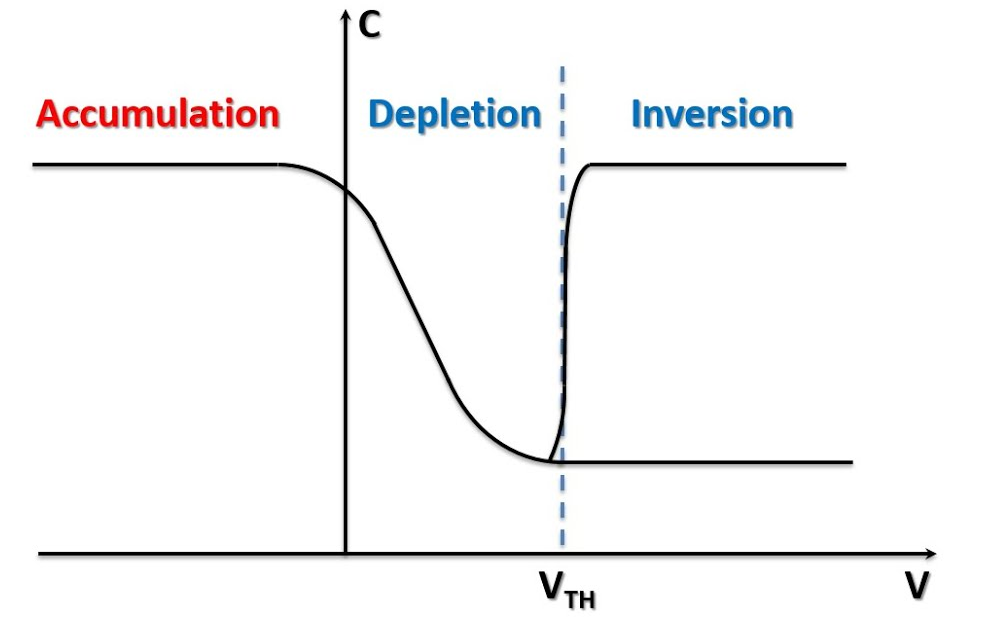
\includegraphics{moscv.png}
\end{figure}

\end{document}
